\documentclass[11pt]{article}
\usepackage[left=2cm,right=2cm,top=2cm,bottom=2cm]{geometry}
\usepackage[utf8]{inputenc}
\usepackage{graphicx}
\usepackage{listings}
\usepackage[english]{babel}
\usepackage{comment}
\usepackage{hhline}
\usepackage{color}
\usepackage{url}
%\usepackage{csquotes}
\usepackage[backend=bibtex,style=verbose-trad2]{biblatex}
\bibliography{test} 
 
\newcommand{\HRule}{\rule{\linewidth}{0.6mm}}
 
\definecolor{codegreen}{rgb}{0,0.6,0}
\definecolor{codegray}{rgb}{0.5,0.5,0.5}
\definecolor{codepurple}{rgb}{0.58,0,0.82}
\definecolor{backcolour}{rgb}{0.95,0.95,0.92}
 
\lstdefinestyle{codestyle}{
    backgroundcolor=\color{backcolour},   
    commentstyle=\color{codegreen},
    keywordstyle=\color{magenta},
    numberstyle=\tiny\color{codegray},
    stringstyle=\color{codepurple},
    basicstyle=\footnotesize,
    breakatwhitespace=false,         
    breaklines=true,                 
    captionpos=b,                    
    keepspaces=true,                 
    numbers=left,                    
    numbersep=5pt,                  
    showspaces=false,                
    showstringspaces=false,
    showtabs=false,                  
    tabsize=2
}
 
\lstset{style=codestyle}

\begin{document}


\begin{titlepage}
\center % Center everything on the page
\HRule \\[0.4cm]
\textbf{\huge Assignment 8}\\[0.3cm] % course name
\textbf{\huge Python and Github}\\[0.3cm]
\HRule \\[1cm]


\textsc{\Large ELP-780}\\[0.4cm] % Course Code
\textsc{\huge Software Lab}\\[1cm] % course name
\textsc{\Large Ravi Singh Thakur}\\ [0.16cm]
\textsc{\Large 2017EET2840}\\[1cm]

\includegraphics[scale=1.25]{logo.jpg}\\[1cm]
\textbf{\Large Indian Institute Of Technology,}\\[0.2cm]
\textbf{\Large Delhi}\\[0.3cm]
{\Large \today}\\[3cm] % Date
\end{titlepage}
\pagebreak

\tableofcontents

\pagenumbering{arabic}
\newpage


\section{Problem Statement 1}
{

\subsection{Problem Statement}
\paragraph{ Find two largest crosses lengths of smart cell grid} 
\begin{itemize}
\item Input a 2D array of strings consisting of DULL and SMART cells and find crosses which will be of odd lengths.
\item Print largest two crosses found in matrix in non increasing order.
\end{itemize}
}

\subsection{Assumptions}
{
\begin{itemize}
\item Cells can either contains S or D character to represent SMART and DULL grid.
\item Dimensions of 2D matrix can not be greater than $105*105$.
\end{itemize}
}




\subsection{Algorithm Steps}
{
\begin{itemize}
\item Take m and n as dimensions from user as input and store S or D in it.
\item Replace S by 1 and D by 0 in this matrix.
\item Take matrx $[-1,0,1]$ to determine cross.
\item Multiply each cell value by this matrix rowwise and columnwise.
\item If column and row sum is equal to 1 then sum it and print it.
\item Repeat above steps for further calculations. 
\end{itemize}





\subsection{Input and Output Format}
{


\textbf{I/O format} 
\begin{itemize}
\item \subsubsection{Input Format}
\begin{itemize}
\item Two space separated values.
\item Input taken as S or D for each cell.
\end{itemize}

\item \subsubsection{Output Format}
\begin{itemize}
\item Two space separated values denoting sizes of two cross.
\end{itemize}
\end{itemize}


}

\subsection{Difficulty faced}
{
\begin{itemize}
\item Determining pattern for cross.
\end{itemize}
}

\subsection{Program Structure}
\begin{center}
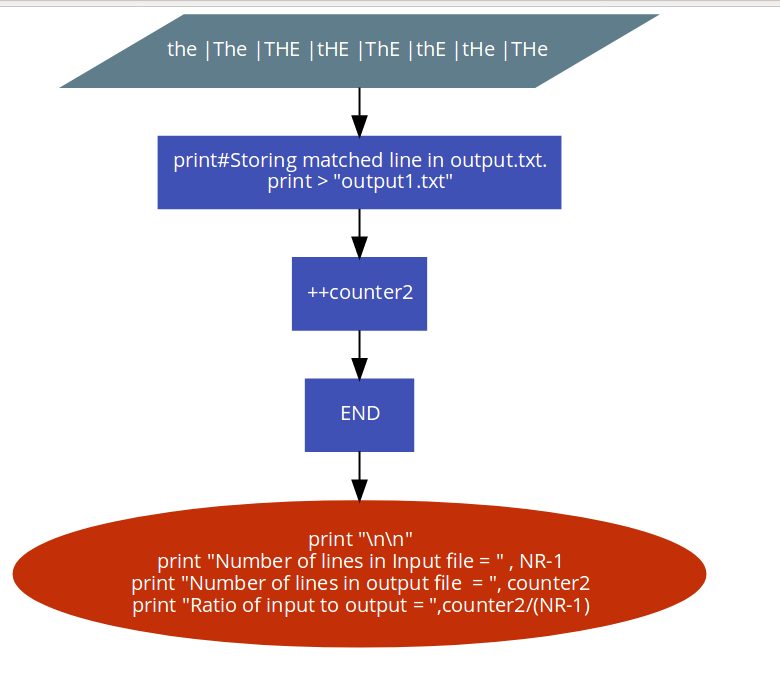
\includegraphics[scale=0.60]{fc2.png}
\end{center}
\newpage


\subsection{Screenshots}
{
\begin{center}
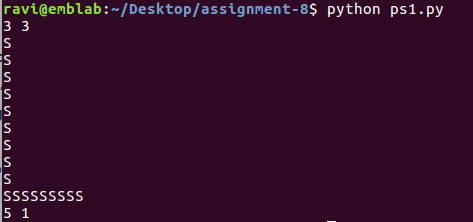
\includegraphics[scale=0.70]{ss1.png}


\end{center}
\newpage
}



\section{Problem Statement 2}
{

\subsection{Problem Statement}
\paragraph{ Rotate keys and values of a string by k.} 
\begin{itemize}
\item Divide alphabets and underscore into three groups and rotate by key and print result.
\end{itemize}
} 

\subsection{Assumptions}
{
\begin{itemize}
\item Keys must be integer.
\end{itemize}
}




\subsection{Algorithm Steps}
{
\begin{itemize}
\item Alphabets and underscore is divided into three groups of tuple as required.
\item Take keys as input for each group to rotate by.
\item Rotate each dictionary by corresponding key.
\item Store result in a list based on dictionary key values.
\end{itemize}

\subsection{Input and Output Format}
{


\textbf{I/O format} 
\begin{itemize}
\item \subsubsection{Input Format}
\begin{itemize}
\item Three space separated keys,one for each group.
\item String is taken as input.
\end{itemize}

\item \subsubsection{Output Format}
\begin{itemize}
\item Decrypted key as output string.
\end{itemize}
\end{itemize}


}

\subsection{Difficulty faced}
{
\begin{itemize}
\item rotate key value pair by key.
\end{itemize}
}

\newpage
\subsection{Program Structure}
\begin{center}
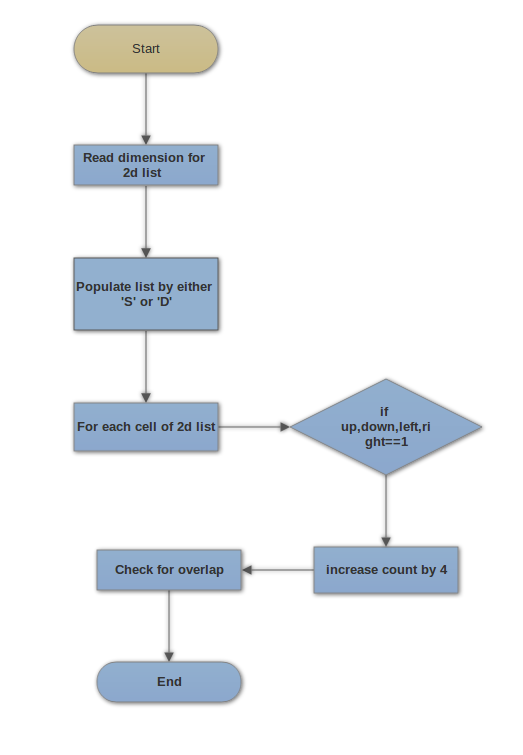
\includegraphics[scale=0.60]{fc1.png}
\end{center}
\newpage

\subsection{Screenshots}
{
\begin{center}
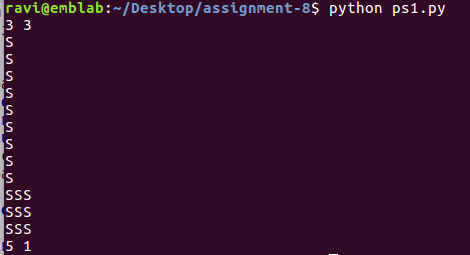
\includegraphics[scale=0.70]{ss21.png}
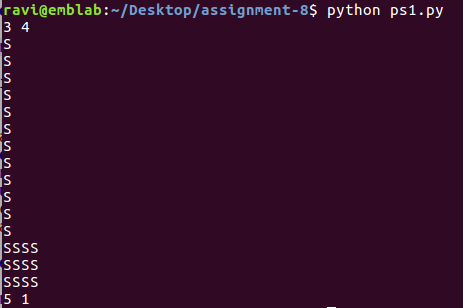
\includegraphics[scale=0.70]{ss22.png}
\end{center}
\newpage
}


\section{Appendix}
{
\textbf{Appendix-A : code for ps1.py}
\lstinputlisting[language=Python]{ps1.py}  

\newpage
\textbf{Appendix-B : code for ps2.py}
\lstinputlisting[language=Python]{ps2.py}

\newpage

}



\begin{thebibliography}{}
\bibitem{} 
https://stackoverflow.com/questions/33554620/rotating-values-in-a-list-python
 
\bibitem{}
https://www.tutorialspoint.com/python/python2darray.htm


 


\end{thebibliography}
\end{document}